\documentclass{article}
\usepackage[round]{natbib}

\usepackage{fullpage}
\usepackage{amsmath}
\usepackage{amsfonts}
\usepackage{graphicx}
\usepackage{color}

\usepackage{xr}
\externaldocument{supplement}

\DeclareMathOperator{\Var}{Var}

\newcommand{\aprcomment}[1]{{\textcolor{blue}{Comment: #1}}}
\newcommand{\E}{\mathbb{E}}

\title{Stabilizing selection, archaic introgression, and the distribution
of shared functional variation}
\author{APR}
\date{\today}

\begin{document}
\maketitle    

\begin{abstract}
    .
\end{abstract}

\section*{Introduction}

Genomic studies have shown that admixture is a common occurrance between
diverged populations and closely related taxa \citep{brandvain2014speciation,
skoglund2015ancient,suvorov2022widespread}, and potentially has been widespread
in primate \citep{tung2017contribution,sorensen2023genome} and hominin
\citep{wolf2018outstanding,peter2020100} evolution. Understanding the effects
of admixture on phenotypic and molecular variation is therefore relevant to
many natural systems, including to studies of the genetic basis of complex
traits and diseases. In particular, archaic introgression in \emph{Homo
sapiens} involving Neanderthals and Denisovans has recently attracted
considerable attention, both in understanding the historical processes leading
to observed distributions of introgressed DNA in present-day populations
\citep{prufer2014complete,villanea2019multiple,chen2020identifying} as well as
its contribution to quantitative traits
\citep{sankararaman2016combined,wei2023lingering}.

After their introduction through admixture, introgressed alleles may be
selected for or against. Some introgressed haplotypes appear to have been
positively selected in modern humans
\citep{huerta2014altitude,racimo2017signatures,enard2018evidence,gower2021detecting},
possibly because such alleles are locally adaptive and provide a fitness
advantage when encountering a novel environment. Despite these cases of
adaptive introgression, introgressed alleles were more likely to have been
negatively selected in modern humans
\citep{harris2016genetic,juric2016strength}. As Neanderthal and Denisovan
population sizes are thought to have been relatively small for hundreds of
thousands of years, theory predicts that they would accumulate deleterious
variation at a faster rate than larger populations. Introgressed haplotypes
would then carry more deleterious variants, which would quickly be selected
against after admixture. \aprcomment{Double check the following statements.} In
mapping the distribution of haplotypes identified as introgressed from
Neanderthals, there is a reduction of Neanderthal-related ancestry in enhancers
and regulatory regions
\citep{petr2019limits,telis2020selection,yermakovich2023long}. This
Neanderthal-allelic depletion, or ``deserts,'' support the hypothesis that
introgressed functional alleles were selected against
\citep{sankararaman2014genomic,sankararaman2016combined}.

There is genetic evidence that early \emph{H. sapiens} reciprocally contributed
to Neanderthal genomes \citep{kuhlwilm2016ancient,hubisz2020mapping}, with
introgression in the reverse direction occurring tens or hundreds of thousands
of years before the Neanderthal-to-human event during the global dispersal of
later humans. This is supported by ``near modern'' \emph{H.  sapiens} outside
of African around 120--100ka or earlier
\citep{schwarcz1988esr,grun2005u,beyer2021climatic}, potentially overlapping
with Neanderthals and providing opportunities for early contacts. While
estimates of the genomic contribution of early \emph{H. sapiens} to
Neanderthals vary \citep{kuhlwilm2016ancient,hubisz2020mapping}, up to 3--5\%
of later Neanderthal genomes may have been contributed through introgression
from humans to Neanderthals. Under the reasoning that \emph{H.
sapiens}-related haplotypes carried fewer deleterious alleles,
human-introgressed DNA would have been favored in Neanderthal genomes. The
replacement of Neanderthal mitochondrial and Y chromosomes by early human
haplotypes supports this model \citep{posth2017deeply,petr2020evolutionary}.

Models for selection against introgressed alleles are often based on load
arguments (in particular, differences in the rate of accumulation of
unconditionally deleterious variation in populations of different sizes) or
hybrid incompatibilities \citep{muller1942isolating}. These arguments are
founded primarily in population genetics theory, with little notion of genetic
variation contributing to phenotypic variation that selection operates on.
Most phenotypic traits are thought to be under stabilizing selection
\citep{sanjak2018evidence,sella2019thinking}, including gene regulation
\citep{gilad2006natural,hodgins2015gene,price2022detecting}. This is relevant
to selection on Neanderthal-introduced alleles in modern humans, as the some of
the strongest signals of selection against such alleles occur in regulatory
regions \citep{sankararaman2014genomic}.

Stabilizing selection on a trait acts to maintain the phenotypic distribution
of that trait near some trait optimum, which is achieved by reducing phenotypic
variation (Figure~\ref{fig:one-pop}A). When the mean phenotype of the
population is close to the phenotypic optimum, classical models predict that
alleles contributing to such a trait are subject to underdominant selection,
i.e., selection against the minor allele at a locus
\citep{robertson1956effect}. This has proven to be a useful model for
understanding allele frequencies of variants contributing to a trait under
stabilizing selection in the single-population setting
\citep[e.g.,][]{keightley1988quantitative, simons2018population,
hayward2022polygenic}.

\begin{figure}[tb!]
    \centering
    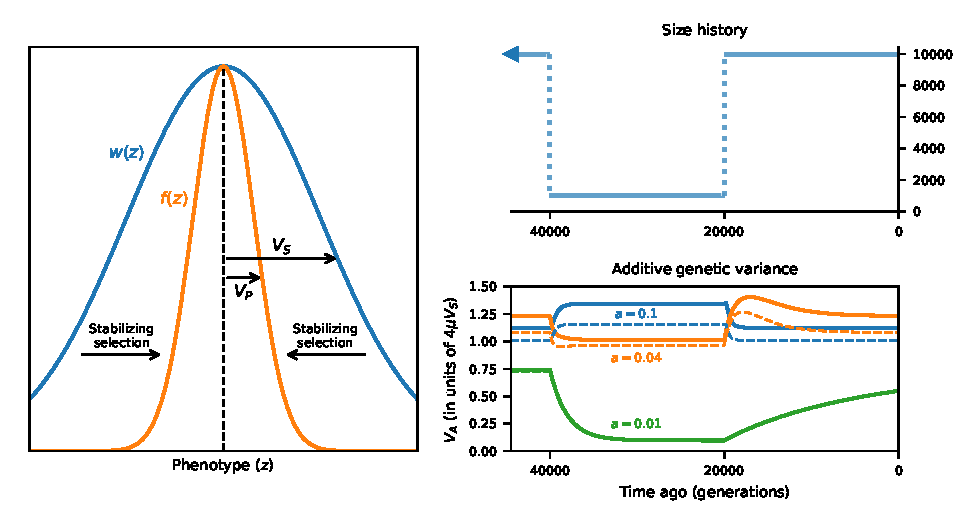
\includegraphics{../figures/one_pop.pdf}
    \caption{
        \textbf{Stabilizing selection and additive genetic variance in one population.}
        \aprcomment{See comparisons to simulations assuming free recombination in
        Figures~\ref{fig:one-popA}--\ref{fig:one-popC}.}
    }
    \label{fig:one-pop}
\end{figure}

In two diverged populations, the genomic architecture of a trait under
stabilizing selection has a higher rate of turnover compared to neutrally
evolving loci \citep{yair2022population}. We might therefore expect an
accumulation of fixed differences between the \emph{H. sapiens} and Neanderthal
branches for alleles contributing to a trait, even when the mean phenotype in
each population is close to the same trait optimum. When alleles that are fixed
in one population are introduced to another population in which they were
previously absent, they will be at low frequency and subsequently selected
against. Likewise, if the ancestral allele is reintroduced to a population
fixed for a derived allele, the ancestral allele will be at low frequency and
will be selected against. In either case we should expect the introgressed
allele, whether ancestral or derived, to be selected against, regardless the
historical relative sizes of the populations involved. This prediction
contrasts with the population-genetics ``load'' model, in which haplotypes with
fewer deleterious variants (such as those from the population with larger
historical size) are favored after introgression in either direction.


\subsection*{Theory and model}

We consider a polygenic trait such that an individual's (additive) genetic
value is the sum over all effects of alleles in their genome, so that for
individual $i$, \(G_i = \sum_l g_{l, i} a_l\), where $a_l$ is the effect size
of the derived allele at locus $l$, and \(g_{l,i}\in\{0,1,2\}\) is their
genotype at that locus (i.e., the number of alleles they carry at that locus).
For unlinked loci, the expected additive genetic variance is \(V_A = \sum_l
2p_l(1-p_l)a_l^2\), where $p_l$ is the allele frequency at locus $l$. We ignore
dominance and epistatic effects, so that \(V_G = V_A\), assuming no linkage.
We can further ingore environmental effects \citep{simons2018population}, so
that the phenotypic variance \(V_P=V_A\).

Stabilizing selection acts to reduce phenotypic variation around the optimum
value $o$, and we assume a Gaussian fitness function so that relative fitness
is given by \(f(G_i | O, V_S) = \exp{(-(G_i - O) / 2 V_S)}\). $V_S$ can be
interpreted as the strength of selection on the trait, where larger $V_S$
implies weaker selection. For a population with mean phenotype at (or very
close to) the optimum, the mean fitness of the population (assuming a roughly
normal distribution of phenotypic values in the population) is
\[\bar{w} \approx \int_{-\infty}^\infty f(G | O, V_S) \mathcal{N}(0, V_G) dG
\approx \left(\frac{V_S}{V_S+V_G}\right)^{1/2}.\]
Thus, as the genetic variance increases, mean fitness among individuals in the
population decreases.

\subsubsection*{Mutation rates and effect sizes}

If all alleles contribute equally to the trait (as \(\pm a\)),
\citet{keightley1988quantitative} showed that the dynamics of $V_G$ can be
approximated with the recursion
\[V_{G,t+1} \approx V_{G,t}\left(1-a^2/2(V_S+V_{G,t})\right)
\left(1-1/2N_e\right) + 2 \mu a^2,\]
where $\mu$ is the per-haploid, per-generation rate of mutation. In the
large-population-size limit, this gives the well-known result
\[\tilde{V_G} \approx 4\mu V_S,\] provided \(V_G \ll V_S\).
Mutations are not expected to each have the same effect size $a$, but
rather will be drawn from some distribution. Here, we will assume mutation
effect sizes are drawn from a normal distribution with mean 0 and given
variance $V_M$.

\subsubsection*{Approximating allelic dynamics via underdominance}

We model the distribution of allele frequencies underlying the trait using
the approximation that alleles are subject to symmetric underdominant
selection \citep{robertson1956effect,keightley1988quantitative}.
For an allele with (heterozygote) additive effect size $a$,
the selection coefficient
\[s\approx \frac{a^2}{2(V_S + V_G)} \approx \frac{a^2}{2V_S},\]
if $V_G \ll V_S$ \citep[e.g.,][]{simons2018population}. Allelic dynamics can
be modeled using the diffusion approximation, where the expected change
in mean allele frequency per generation is
\[\E[M_{\delta_p}] \approx -s p(1-p)(1-2p),\]
and the expected change in variance of the allele frequency per generation is
\[\E[V_{\delta_p}] \approx \frac{1}{4N_e}p(1-p).\]
%From this, because $s$ is always positive for any $a\not=0$, we see that
%selection pushes allele frequencies to zero if $p<1/2$ and to one if $p>1/2$.
%$p=1/2$ is an unstable equilibrium.

We extend the moments-based solution for the sample site-frequency spectrum
(SFS) \citep{jouganous2017} to include underdominance with given selection
coefficient $s$ (\(=a^2/2(V_S+V_G)\)). The contribution of alleles with effect
size $a$ to the total genetic variance $V_G$ is then found by computing the
expected pairwise diversity from the SFS (with sample size $n$, $\Phi_n$), as
\[V_{G,a} = 2a^2\sum_{j=1}^{n-1}\frac{j(n-j)}{n(n-1)}\Phi_n(j|a,\mu_a)da.\]
Here, $\mu_a$ is the mutation rate of alleles with effect size $a$. The total
genetic variance is then 
\[V_G=\int_{-\infty}^\infty V_{G,a}\mathcal{N}(0,V_M).\]

Figure~\ref{fig:one-pop}C shows that if $V_G$ is non-negligible compared to
$V_S$, ignoring $V_G$ and using $s=a^2/2V_S$ leads to lower estimates of
additive genetic variance. When mutation rates are large so that $V_G$ is not
small compared to $V_S$, using $s=a^2/2(V_S+V_G)$ provides estimates of $V_G$
that closely match simulations assuming free recombination between loci
(Figure~\ref{fig:toy-admixture}C,D). Because $V_G$ can change over time, this
means that $s$ is no longer constant, but can change due to factors such as
non-constant demography that increase or reduce $V_G$.

\begin{figure}[tb!]
    \centering
    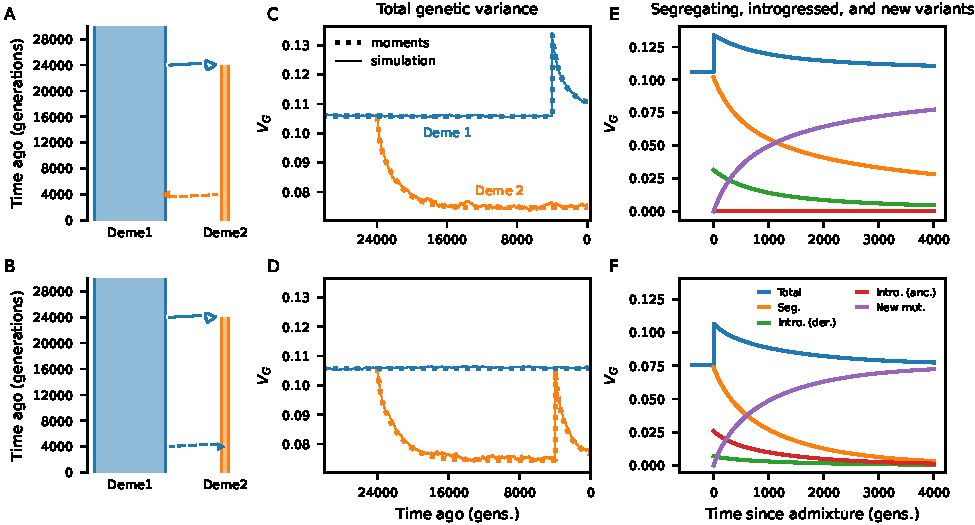
\includegraphics{../figures/reciprocal_admixture.pdf}
    \caption{
        \textbf{}
    }
    \label{fig:toy-admixture}
\end{figure}

\subsubsection*{Demographic history}

Our numerical solution for the SFS allows for non-constant population size
histories, population splits, continuous migration, and admixture. In this
study, we consider relatively simple scenarios involving population splits with
subsequent introgression events. We focus on parameter regimes relevant to
human-Neanderthal history. In the simplest model -- which is not meant to
perfectly match any particular known or inferred history, but instead
demonstrate the effect of reciprocal introgression following population
divergence -- a population of size $N_e=10\,000$ splits into two, on remaining
size $10\,000$ and the other shrinking to size $1\,000$. They remain isolated
for $2N_e$ generations (or 500 thousand years, assuming an average generation
time of 25 years) and then introgression occurs from one branch to the other,
contributing $5\%$ ancestry to the recipient population
(Figure~\ref{toy-admixture}A,B).

The second model is meant to more closely resemble inferred human-Neanderthal
history, in which the ancestral population of size $N_e=10\,000$ splits into
the human and Neanderthal branches. At 250ka, an early human-to-Neanderthal
introgression contributes $5\%$ ancestry to Neanderthals. The human branch
shrinks to size $1\,000$ 60ka, followed by exponential growth to $20\,000$ at
present time. Neanderthals contribute $2\%$ ancestry to this bottlenecked and
expanding human population at 50ka, after which their branch ceases
(Figure~\ref{fig:neand-to-human}A).

In each scenario, we track genetic diversity and phenotypic variance before and
after admixture to understand allele frequency and haplotype dynamics. The
trait optimum is $0$ in all branches, and the strength of selection $V_S=1$
remains constant. \aprcomment{Justified by equivalence under rescaling
\citep{simons2018population}.}

\section*{Results}

\subsection*{Additive genetic variance after admixture}

We expect genetic variance to increase after introgression. The amount that
genetic variance increases depends on the allelic differences accumulated
between populations and the effects of those alleles. Assuming no linkage,
dominance or epistasis, \(V_G=\sum_l 2p_l(1-p_l)a_l^2\). After admixture, with
proportion $f$ contributed by the source population (labeled 0) into the focal
population (labeled 1), \(p_l = fp_{l,0} + (1-f)p_{l,1}\). Plugging into the
expression for $V_G$, and after some simple algebra (Appendix~AX), we can
express the expected genetic variance directly after admixture as \[V_G =
fV_{G,0} + (1-f) V_{G,1} + 2f(1-f)\sum_l F_{2,l} a_l^2,\] where $F_2 = (p_0 -
p_1)^2$ is the squared difference in allele frequencies at a locus
\citep[e.g.,][]{peter2016admixture}. This result is known
\citep[e.g.,][]{tufto2000quantitative}, showing that additive variance is equal
to that in the source populations weighted by their contributions, plus a term
that depends on the divergence at trait-affecting loci between the populations
weighted by the quadratic factor $2f(1-f)$.

In general, $F_2$ at a given locus will depend on the demographic history
relating the two populations and the effect size at the locus due to selection
on the trait. In the infinitesimal limit, involving many loci each of
vanishingly small effect, dynamics at a given locus will be approximately
neutral, so that $F_2$ depends only on the demography. In this case
\begin{align*}
    V_G & \approx f V_{G,0} + (1-f) V_{G,1} + 2f(1-f)\mathbb{E}[F_2] \sum_l a_l^2 \\
    & = f V_{G,0} + (1-f) V_{G,1} + 2f(1-f)\mathbb{E}[F_2] n_m V_M,
\end{align*}
where $V_M$ is the variance of effect sizes of new mutations (assuming the mean
is zero). 

For $a \not\approx 0$, assuming neutral evolution will tend to overestimate
$F_2$ compared to underdominant selection. We can compute expected $V_G$ both
before and after admixture using the diffusion approximation for the joint SFS
with underdominance. Comparing to simulations with free recombination between
loci (Appendix~AY), we find that this provides an excellent fit to average
observed $V_G$ over time (Figure~\ref{fig:toy-admixture}C,D). Following an
initial rapid increase in $V_G$ due to admixture, it decays back to the
steady-state expectation relatively rapidly.

\begin{itemize}
    \item Benefit of SFS -- partition by frequency classes (prev. seg vs introgressed)
    \item VG from all both previously segregating and introgressed alleles decays,
        replaced by VG due to new mutations
    \item Dividing VG from introgressed alleles into introduced derived vs reintroduced
        ancestral alleles shows the effect of differences in population sizes
\end{itemize}

\subsection*{Recurrent introgression and non-constant population size}

\begin{figure}[t!]
    \centering
    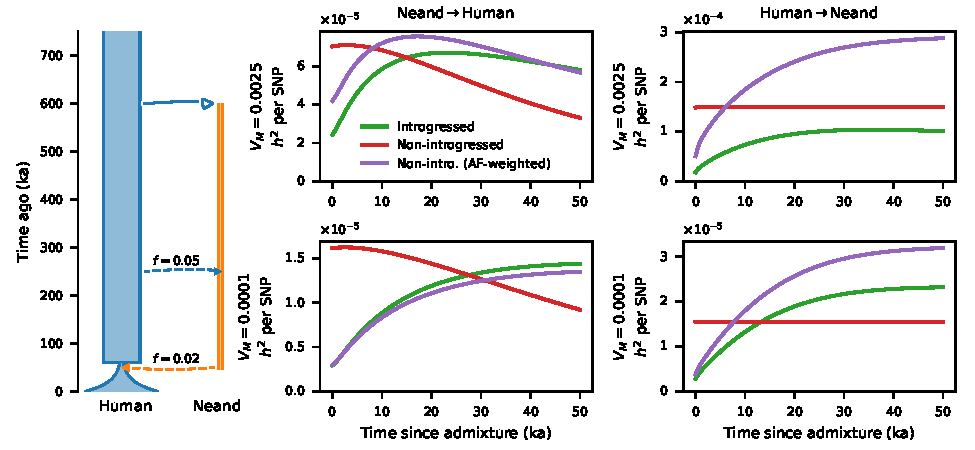
\includegraphics{../figures/neanderthal_admixture.pdf}
    \caption{
        \textbf{}
    }
    \label{fig:neand-to-human}
\end{figure}

\begin{itemize}
    \item In the demographic model more closely resembling inferred history
        connecting humans and Neanderthals (Figure~\ref{fig:neand-to-human}A),
        we see that demographic history and the distribution of effect sizes
        of new mutations impact $V_G$
    \item Additive genetic variance increases after introgression in both directions,
        which is expected to result in a period of decreased mean fitness
    \item Population contractions decrease $V_G$, as the increased rate of drift
        reduces diversity at loci underlying the trait
    \item TODO: compare to linked simulations
\end{itemize}

\begin{figure}[t!]
    \centering
    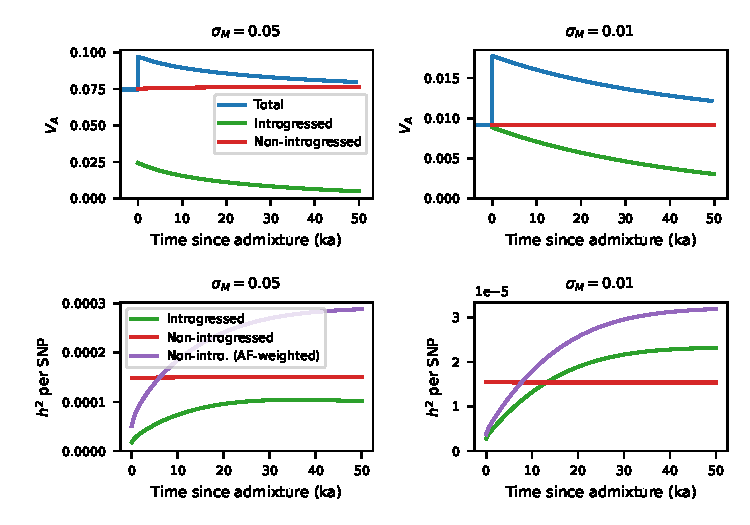
\includegraphics{../figures/human_admixture.pdf}
    \caption{
        \textbf{}
    }
    \label{fig:human-to-neand}
\end{figure}

\begin{itemize}
    \item Because we know if a mutation was previously segregating in the population
        receiving migrants, we can partition variation by contributions from
        segregating vs introgressed variants (whether introduced derived mutations
        or reintroduced ancestral mutations)
    \item At low introgression proportions, as here, the majority of $V_G$ is still
        contributed by previously segregating mutations, which is then expected to
        be steadily replaced by new mutations (Figure 2). $V_G$ due to introgressed
        variation decays monotonically over time (Figure~\ref{fig:neand-to-human}C,D)
    \item While the total $V_G$ due to introgressed variants decays, we can also
        consider the average contribution of introgressed vs non-introgressed SNPs
        to $V_G$ ($h^2$ per SNP) -- at least for this demographic model and
        DES, the contribution per SNP of introgressed variants is initially lower
        than those of previously segregating variants. These contributions change
        over time, in a way that depends on both the genomic architecture underlying
        the trait and demography
    \item This dependence on both architecture and demography is apparent when
        comparing to $V_G$ contributed by introgressed and non-introgressed variants
        in the early human-to-Neanderthal admixture (Figure~\ref{fig:human-to-neand})
        -- here, again the contribution
        from introgressed variants to $V_G$ decays monotonically, but depending on
        the distribution of effect sizes, relative per-SNP $h^2$ changes over time
        (though in these cases introgressed $h^2$ per SNP remains lower than
        non-introgressed, when considering mutations at matched allele frequencies)
\end{itemize}

\subsection*{The effects of linkage}

\begin{itemize}
    \item So far, we have considered model and simulation without linkage -- in this
        case, the underdominance model provides an excellent approximation
    \item Including linkage between sites dramatically complicates things, making
        theorical or analytical progress difficult
    \item To explore the effects of linkage, we used individual-based simulations
        with a single large chromosome of size 1 Morgan, and varried the total
        mutation rate per haploid and the variance of effect sizes of new mutations
    \item We'll highlight two effects of linkage
        \begin{itemize}
            \item Deviations from expected $V_G$, as well as more complicated
                short-term dynamics after admixture
            \item The reduction in introgressed ancestry in the regions surrounding
                trait-affecting alleles
        \end{itemize}
\end{itemize}

\subsubsection*{Effects of linkage on expected genetic variance}

\begin{figure}[t!]
    \centering
    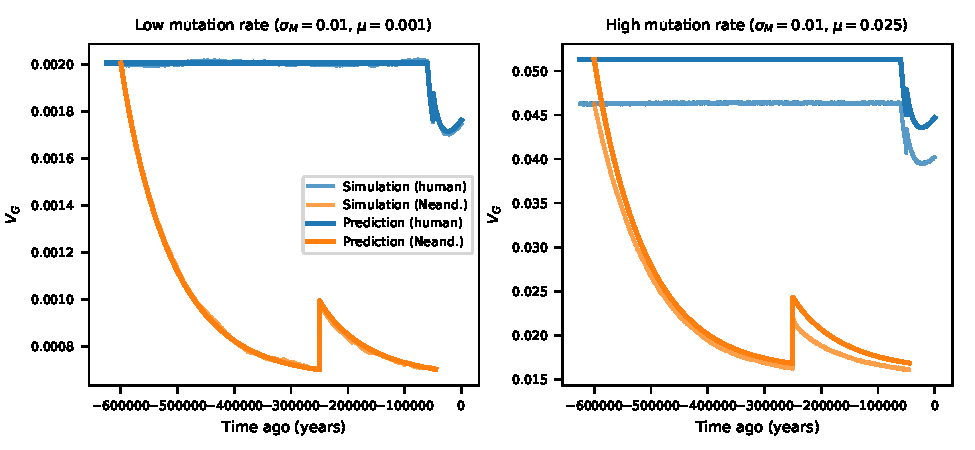
\includegraphics{../figures/model_comparison.SD_0.01.mu_0.001_0.025}
    \caption{}
    \label{fig:linkage-deviations}
\end{figure}

\begin{itemize}
    \item Stabilizing selection reduces $V_G$ by selecting against minor alleles
        (underdominance), but with linkage it can also reduce $V_G$ by selecting
        for haplotypes that carry opposite effect alleles that cancel out -- this
        creates LD between positive and negative effect alleles at linked loci,
        known as the Bulmer effect \citep{}
    \item Thus, $V_G$ in simulations with linkage deviate from predictions
        assuming underdominance alone
    \item The severity of this deviation depends on a number of factors: mean
        recombination rate between trait-affecting loci, the total mutation rate,
        the effect sizes (and distribution of effect sizes of new mutations)
    \item In general, lower mutation rates imply lower total $V_G$, lower polygenicity,
        and therefore higher recombination rates between trait-affecting alleles --
        we therefore expect this deviation to be exacerbated with higher mutation
        rates (all else being equal)
\end{itemize}

\subsubsection*{Reduction of introgressed ancestry surrounding an introgressed trait-affecting allele}

\begin{itemize}
    \item Because introgressed trait-affecting alleles are selected against as the
        minor allele, linkage will also remove introgressed ancestry segments in the
        regions surrounding the selected alleles
    \item The expected reduction in introgressed ancestry proportions surrounding
        functional alleles will depend on the effect size of the trait-affecting allele
        and the probability of recombination surrounding that site
    \item We can consider first a deterministic model of the dynamics of introgressed
        allele frequencies at and around an introgressed functional allele -- this
        model considers a single trait-affecting locus, ignoring any effects of
        interference between selected alleles
        \begin{itemize}
            \item Consider a site with fixed differences between the two populations
                (the derived allele is fixed in one, lost in the other)
            \item At the functional site itself, with admixture proportion $f$ from the
                minor parental ancestry, the initial frequency of the derived allele
                is $p_0=f$ or $p_0 = 1-f$, if the derived allele was fixed in the 
                major parental ancestry population
            \item In one generation, the expected allele frequency at the selected locus
                is \[p_{t+1} \approx p_t - s p_t(1-p_t)(1-2p_t),\] where $s=a^2/2V_S$
            \item As discussed earlier, if $p_0<1/2$, $p_t\rightarrow0$, and if $p_0>1/2$,
                $p_t\rightarrow1$ as $t\rightarrow\infty$
            \item Consider a neutral locus separated from the selected locus by
                recombination probability $r$. Initially, the expected frequency
                of introgressed ancestry at that locus is $q_0=f$
            \item The linked ancestry frequency will change due to selection acting on
                the trait-affecting locus, depending on the strength of selection
                at that locus and the level of linkage disequilibrium between
                the two loci
            \item $D=Cov(p,q)$ is the standard covariance measure of LD between loci,
                and $q$ is expected to change as \[q_{t+1} \approx q_t - s D_t(1-2p_t)\]
            \item $D$ also changes over time, due to both selection and recombination,
                so that \[D_{t+1} \approx D_t - r D_t - s D_t (1-2p_t)^2\]
            \item Initially, $D_0 = \pm f(1-f)$, with $D$ being positive if $p_0=f$
                and negative if $p_0=1-f$
            \item Together, this forms a nonlinear system of equations for the
                deterministic change in allele frequencies at the two loci (one
                selected, one neutral) and LD between them -- note that this is
                deterministic in the infinite population size limit
        \end{itemize}
    \item Using this model, we can predict how allele frequencies and LD are expected
        to change over time after admixture, for a given effect size $a$ and 
        recombination rate $r$ (Figure~\ref{fig:linkage-pred}A,B)
    \item As expected, lower effect sizes result in a slower reduction in introgressed
        ancestry frequency, while higher recombination rates more quickly decouple
        the linked ancestry from the selected allele
    \item Thus, the expected reduction in introgressed ancestry is largest for
        larger effect sizes (Figure~\ref{fig:linkage-pred}C), and LD between the
        selected and linked neutral alleles is largest for neutral sites closest
        to the selected allele (Figure~\ref{fig:linkage-pred}D)
\end{itemize}


\begin{figure}[t!]
    \centering
    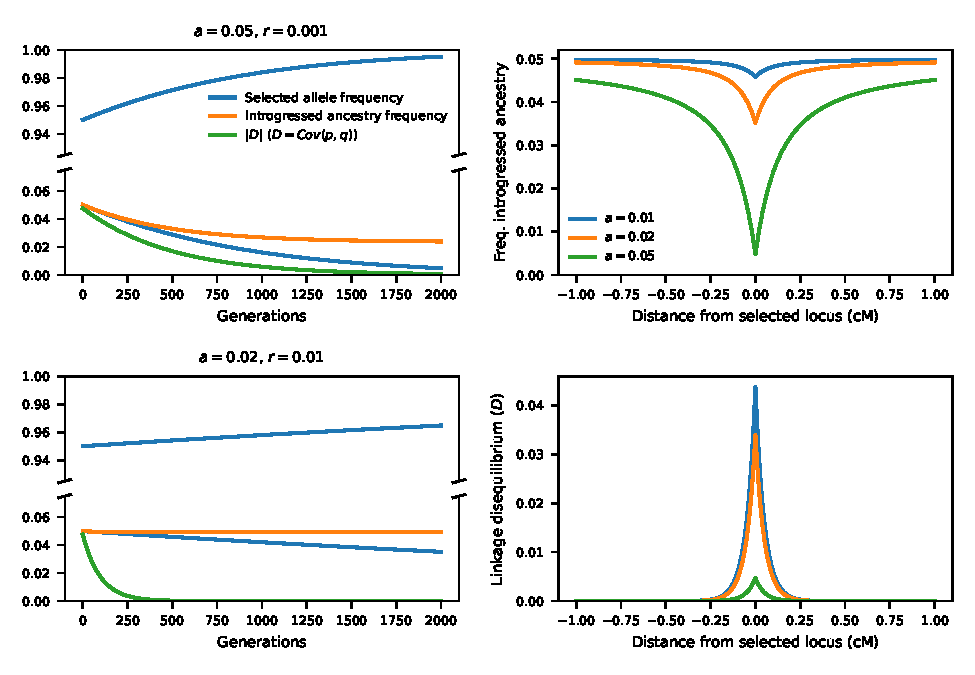
\includegraphics{../figures/linkage_predictions.pdf}
    \caption{
        \textbf{}
        \aprcomment{Linked allele frequency should always be minor, and labeled
        introgressed ancestry frequency}
    }
    \label{fig:linkage-pred}
\end{figure}

\begin{itemize}
    \item To explore the accuracy of this two-locus model, we compared to
        simulations using the demographic model shown in
        Figure~\ref{fig:toy-admixture}A with introgression fraction $f=0.05$.
        We simulated a single 1 Morgan
        chromosome, with all mutations having effect sizes $\pm a$ ($a=0.02$ or
        $0.05$, with equal probability of being trait-increasing or decreasing)
        and varying the total mutation rate ($\mu=0.001$, $0.0025$, and $0.01$)
    \item For each mutation that was fixed in one population and absent in the
        other (either fixed in the minor or major ancestry population), we
        determined the average introgressed ancestry surrounding those introgressed
        alleles (Figure~\ref{fig:linkage-sim})
    \item The deterministic model provides a very good approximation for linked
        introgressed ancestry when the mutation rate is small
    \item As the mutation rate increases, polygenicity increases so that
        trait-affecting alleles are more densely distributed along the chromosome --
        deviations from the deterministic model are due to interference between
        tightly linked trait-affecting alleles. For the highest mutation rate shown
        here, there will be many trait-affecting alleles within the 1 cM window
        around any focal SNP
\end{itemize}

\begin{figure}[t!]
    \centering
    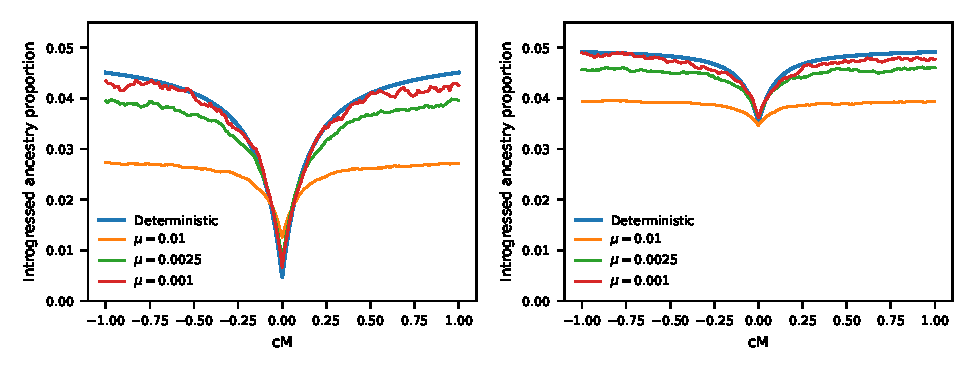
\includegraphics{../figures/linkage_simulation.pdf}
    \caption{
        \textbf{}
    }
    \label{fig:linkage-sim}
\end{figure}

\begin{figure}[t!]
    \centering
    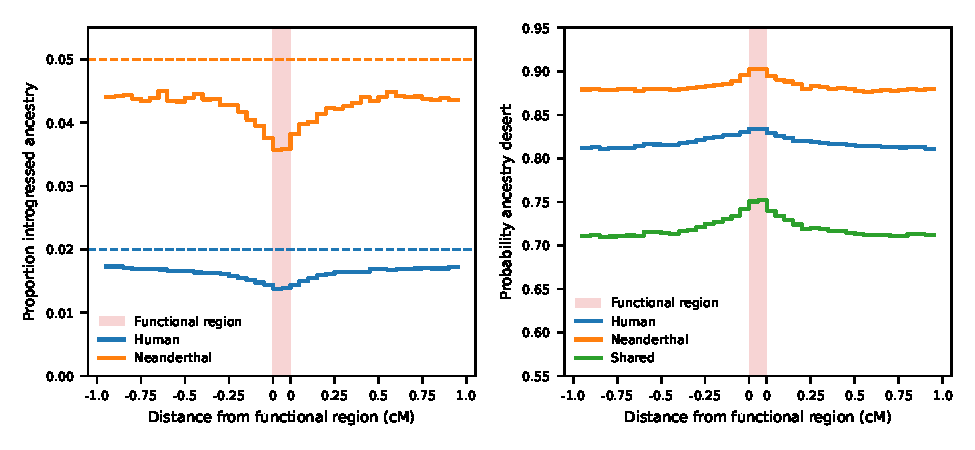
\includegraphics{../figures/introgression_deserts.SD_0.02.pdf}
    \caption{
        \textbf{}
    }
    \label{fig:deserts}
\end{figure}

\section*{Discussion}

\begin{itemize}
    \item Stabilizing selection with a constant optimum is an appropriate
        null model for the dynamics of trait variation and selection on
        alleles underlying those traits
    \item Stabilizing selection results in population genetic predictions
        for patterns of introgressed variation in and around functional
        regions that differ from both load- and incompatibility-based arguments
        \begin{itemize}
            \item Load-based models predict that haplotypes from the less ``loaded''
                population will be favored under introgression in either direction
                -- thus, regions of depleted ancestry after introgression in one
                direction will not be expected to also be introgressed ancestry
                deserts after admixture in the opposite direction
            \item \citet{mueller1942} originally pointed out that hybrid
                incompatibilities should not form at single loci -- classical
                incompatibilities require two or more loci, which are not
                expected to be tightly linked to one another. Thus, under a
                model of hybrid incompatibilities, the minor parent ancestry
                is again selected against, but those loci will be in different
                regions. Again, deserts are therefore not expected to overlap
                if selection is largely due to incompatibilities
            \item Instead, stabilizing selection causes introgressed DNA to be
                depleted at the same loci under bi-directional gene flow
                (could be thought of as single-locus incompatibility effects --
                but these are not incompatibilities in the classical sense,
                as the same effects occur even without admixture)
            \item A prediction we could make is that, if current models are correct
                that there has been introgression in both directions between
                \emph{H. sapiens} and Neanderthals, introgressed ancestry deserts
                should overlap with each other more often than expected by chance
            \item See Figure~\ref{fig:ancestry-deserts}
        \end{itemize}
    \item Shared deserts are most likely to form where moderate- or large-effect
        alleles have fixed in one population or the other -- this could provide
        an approach to map\dots?
    \item Selection in structured populations with ongoing migration or
        meta-populations -- SFS approach can handle this -- prospects for the
        future
    \item Some conjectures about hybrid zones
    \item Pleiotropy\dots!!!
\end{itemize}

\section*{Methods}

\subsection*{Computing expected genetic variance using the diffusion approximation}

\subsection*{Simulations with free recombination}

\subsection*{Individual-based simulations with linkage}

\bibliographystyle{genetics}
\bibliography{manuscript}

\section{Appendix}

\subsection{Additive genetic variance after admixture}

Suppose two population (labeled 0 and 1) diverged some time in the past and
then admix in proportions $f$ and $1-f$.

Assuming no linkage, dominance or epistasis (so \(V_G=V_A\)),
\[V_G = \sum_l 2p_l(1-p_l)a_l^2 = \sum_l \pi_l a_l^2,\]
where $\pi$ denotes expected pairwise diverisity.
At a given locus (dropping the $l$), after admixture the allele frequency is
\[p=f p_0 + (1-f) p_1,\]
so that
\begin{align*}
    2p(1-p) & = 2(f p_0 + (1-f) p_1)(1 - f p_0 - (1-f) p_1) \\
    & = f^2 2p_0(1-p0) + (1-f)^2 p_1(1-p1) + 2f(1-f) (p_0(1-p_1) + p_1(1-p_0)) \\
    & = f^2 \pi_{0,0} + (1-f)^2 \pi_{1,1} + 2f(1-f)\pi_{0,1}.
\end{align*}

Plugging in to the definition for $V_G$, we get after admixture
\[V_G = f^2 V_{G,0} + (1-f)^2 V_{G,1} + 2f(1-f)\sum_l \pi_{0,1,l}a_l^2.\]
We can write $\pi_{0,1}$ at a given locus in terms of $\pi_{0,0}$, $\pi_{1,1}$,
and $F_2(0,1)=(p_0-p_1)^2$ as \citep{peter2016admixture}
\[\pi_{0,1} = F_2(0,1) + \frac{1}{2}\pi_{0,0} + \frac{1}{2}\pi_{1,1}.\]
Then
\begin{align*}
    V_G & = f^2 V_{G,0} + (1-f)^2 V_{G,1} + 2f(1-f)\sum_l \left[F_{2,l}(0,1)
    + \frac{1}{2}\pi_{0,0} + \frac{1}{2}\pi_{1,1}\right] a_l^2 \\
    & = f^2 V_{G,0} + (1-f)^2 V_{G,1} + 2f(1-f)\left[\frac{1}{2}V_{G,0} 
    + \frac{1}{2}V_{G,1} + \sum_l F_{2,l}(0,1)a_l^2\right] \\
    & = \left(f^2 + f(1-f)\right) V_{G,0} + \left((1-f) + f(1-f)\right)V_{G,1}
    + 2f(1-f) \sum_l F_{2,i}(0,1)a_l^2 \\
    & = f V_{G,0} + (1-f)V_{G,1} + 2f(1-f)\sum_i F_{2,l}(0,1)a_l^2.
\end{align*}


\begin{figure}[tb!]
    \centering
    %\includegraphics{}
    \caption{
        \textbf{Dynamics of additive genetic variance in two populations with admixture.}
        Coupled with the equations for the decay of $V_G$ due to drift and selection,
        and the increase in $V_G$ through mutation, show that the expected dynamics
        are matched by simulations without linkage.
    }
    \label{fig:VG_dynamics}
\end{figure}

\subsection{Dynamics of introgressed alleles}

\subsection{Reciprocal depletion of functional variation}

While incompatibilities require two or more loci (Morgan, 1942), introgression
with stabilizing selection can create the appearance of a single-locus
incompatibility via underdominance\dots


\end{document}
